% 2024-09-?? EFMI STC Timisoara, Romania conference paper presentation
% 10 minutes presentation.

%\documentclass[aspectratio=43]{beamer}
%\documentclass[aspectratio=169]{beamer}
\documentclass[aspectratio=1610,12pt]{beamer}

\usepackage[english]{babel}
\usepackage{booktabs} % fancy tables
\usepackage{tabulary} % tables with auto column length 
\usepackage{hyperref}
\usepackage{siunitx}

\usetheme{imise}
\author{\emph{Konrad Höffner}, Hannes Raphael Brunsch, Franziska Jahn,\\Prof. Alfred Winter}
%\title{The SNIK Ontology of Information Management in Hospitals}
\title{\large Visualising Paths for Exploratory Search\\in the Health IT Ontology}
\date{September 2?, 2024}%, EFMI STC 2024}
\def\address{Härtelstraße 16-18, 04107 Leipzig, Raum 227}
\def\email{konrad.hoeffner@imise.uni-leipzig.de} 
\def\telephone{+49 341 97 16322}


\newcommand{\imageslide}[4][]
{
\newgeometry{margin=0cm,top=1em}
\begin{frame}[plain]{~~~~#2}
\vspace{0.2em}
\centering\includegraphics[width=0.995\textwidth,height=0.95\textheight,keepaspectratio]{#3}
\\#1
\note{#4}
\end{frame}
\restoregeometry
}

\newcommand{\imageslidebare}[1]
{
\newgeometry{margin=0cm,top=1em}
\begin{frame}[plain]
\centering\includegraphics[width=0.995\textwidth,height=0.995\textheight,keepaspectratio]{#1}
\end{frame}
\restoregeometry
}

\begin{document}

\begin{frame}
\titlepage
\end{frame}

\imageslide{The Health IT Ontology}{img/2024-05-hito\_diagram.pdf}{}{}
%\imageslide{Exploration Options: RDF Browser}{img/rickview-hito.png}{}{}
\imageslidebare{img/cscmedchart-lodview.pdf}
\imageslide{Linked Data Browser}{img/cscmedchart-lodview.pdf}{}{}
\imageslide{Faceted Search}{img/hitofaceted.png}{}{}
\imageslidebare{img/idea.pdf}


\newgeometry{margin=0cm,top=1em}
\begin{frame}[plain]{~~~~Domain}
% Information Management in Hospitals is a core topic for students of medical computer science.
% Unfortunately, there are many different views of the domain, whose relationship is often unclear, and the terminology is full of synonyms and homonyms.
% So this domain is difficult to learn for students. 
\end{frame}
\restoregeometry

%\imageslide{Synonyms}{img/wordcloud-synonym.png}{}{}

%\imageslide{Meta Model}{img/metamodel9s.pdf}{}{}

%\imageslide{Modelling Example}{img/bb-cio.pdf}{}{}

\newgeometry{margin=0cm,top=1em}
\begin{frame}[plain]{~~~~Transformation}
%\centering%\includegraphics[width=0.7\textwidth,keepaspectratio]{img/5star.png}
\end{frame}
\restoregeometry

%\newgeometry{margin=0cm,top=1em}
\iffalse
\begin{frame}[plain]{~~~~Storage/Query, Author, Interlink \& Browse}
\begin{columns}[t]
\column{.5\textwidth}
\centering
%\includegraphics[width=\textwidth]{img/virtuoso.png}
%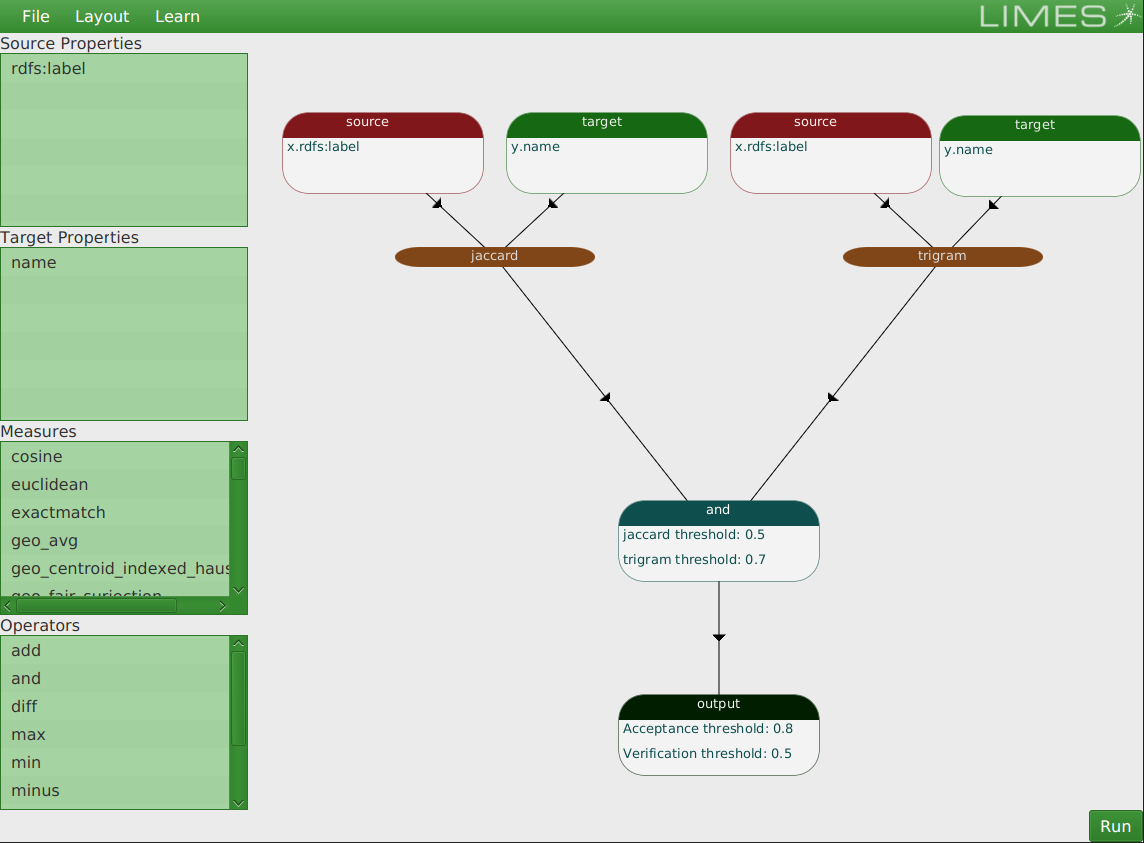
\includegraphics[width=\textwidth]{img/limes.png}
\column{.5\textwidth}
\centering
%\includegraphics[width=\textwidth]{img/ontowiki.png}
%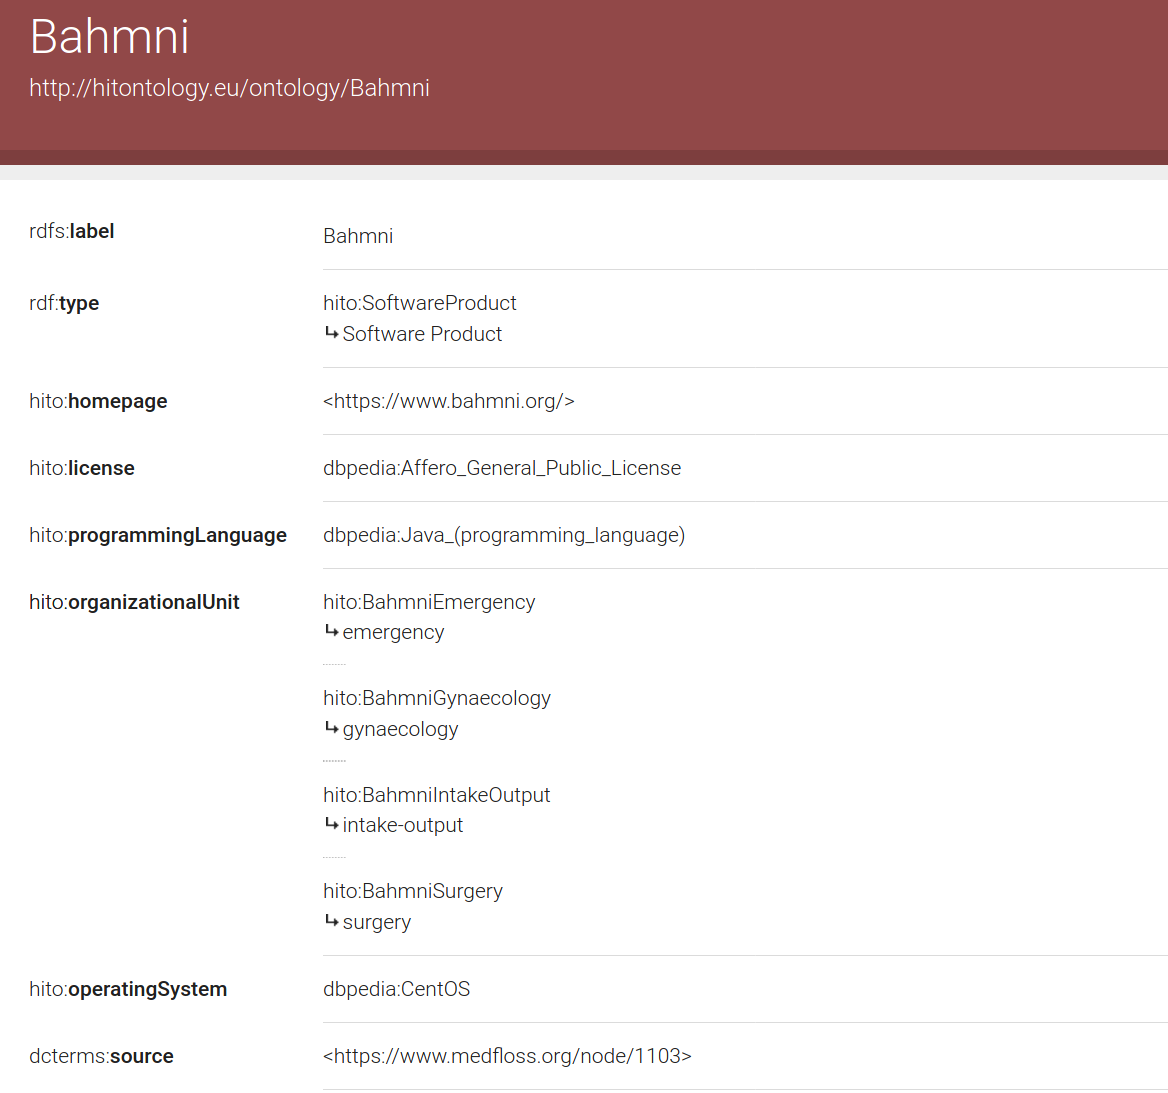
\includegraphics[width=\textwidth]{img/lodview.png}
\end{columns}
\end{frame}
\fi
%\restoregeometry

%\imageslide{Search \& Exploration: SNIK Graph}{img/snik-graph-full.png}{}{}

%\imageslide{Extraction}{img/5star.png}

\iffalse
\begin{frame}{Example Slide}
\begin{itemize}
\item 
\item 
\item 
\item 
\end{itemize}
\end{frame}

\begin{frame}[fragile]{Fragen?}
\begin{itemize}
%\item Diese Präsentation \url{https://github.com/KonradHoeffner/latex/releases/download/colloquium/colloquium.pdf}
\vspace{0.5em}%here it works as intended
\item Überblick \url{http://www.snik.eu}
\item Visualisierung \url{http://www.snik.eu/graph}
\item SPARQL Endpunkt \url{http://www.snik.eu/sparql}
\item RDF Browser \url{http://www.snik.eu/ontology}
\item Evaluation \url{http://www.snik.eu/evaluation}
\item Twitter \url{https://twitter.com/snik\_proj}
\item Technisches Blog \url{https://imise.github.io/snik-ontology}
\item GitHub Organisation mit Ticketsystem \url{https://github.com/imise}
\end{itemize}
\end{frame}
\fi

\end{document}
